\documentclass[9pt]{article}
\usepackage[spanish]{babel}
\usepackage[utf8]{inputenc}
\usepackage{graphicx}
\graphicspath{{media/}}
%\renewcommand{\familydefault}{\sfdefault}
\begin{document}
\title{Proyecto 1}
\author{Carlos Gerardo Acosta Hernández \\ Andrea Itzel González Vargas \\ Luis Pablo Mayo Vega}
\date{Redes de Computadoras\\Facultad de Ciencias, UNAM}
\maketitle

\section*{Reporte}

\subsection*{Diagrama de Red}

\subsection*{DNS}

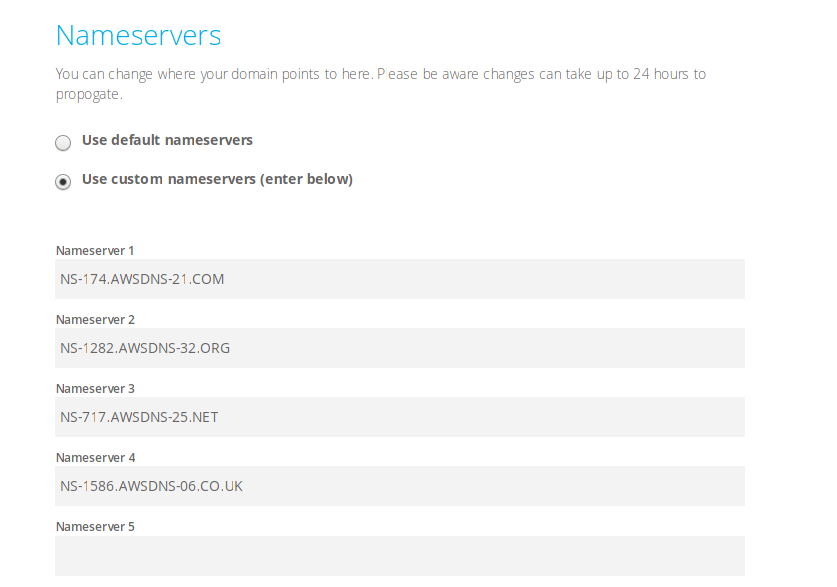
\includegraphics[width=\textwidth]{nameservers}
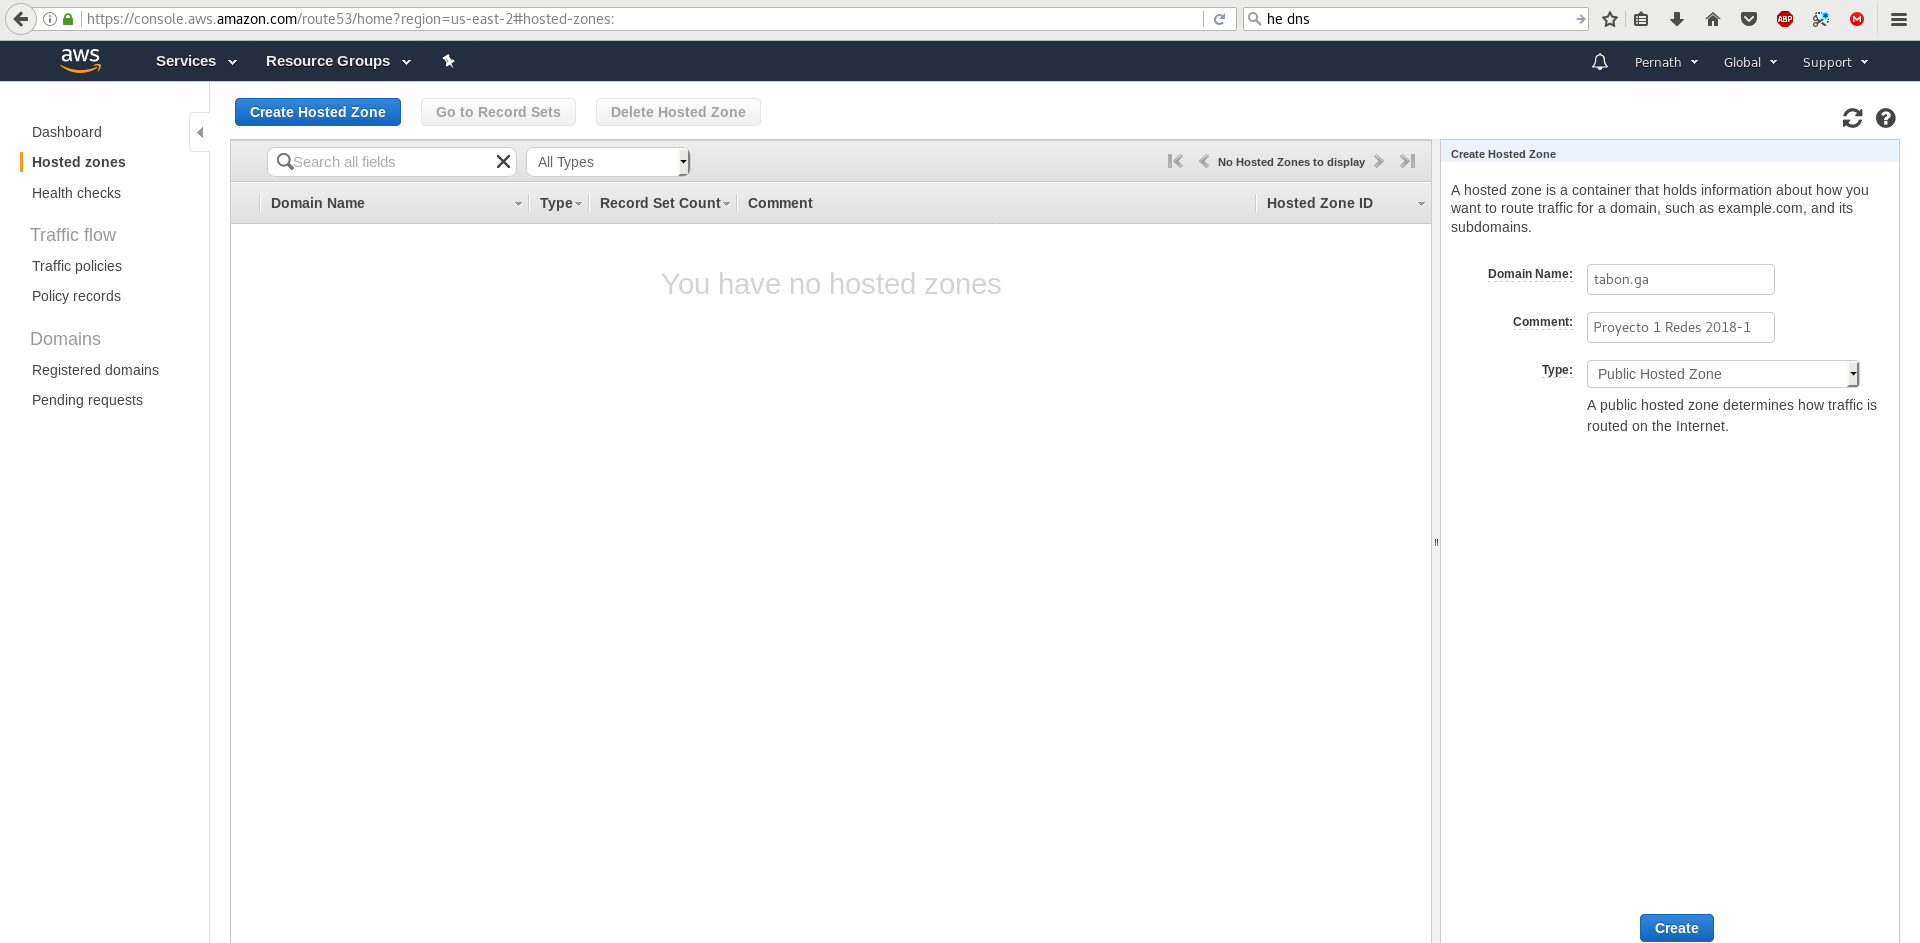
\includegraphics[width=\textwidth]{DNS_management}
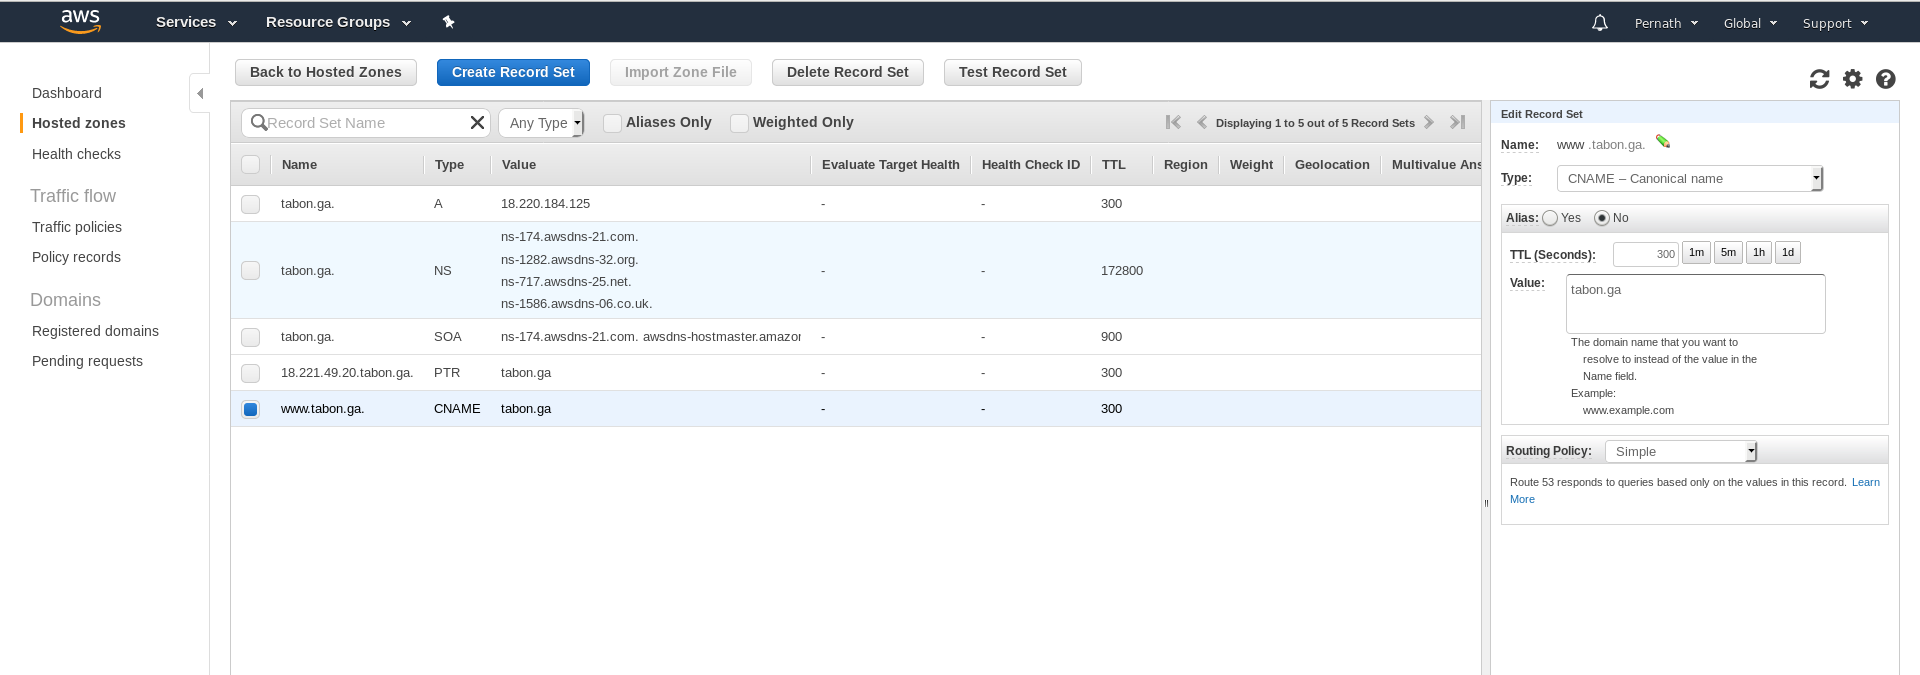
\includegraphics[width=\textwidth]{CNAME}
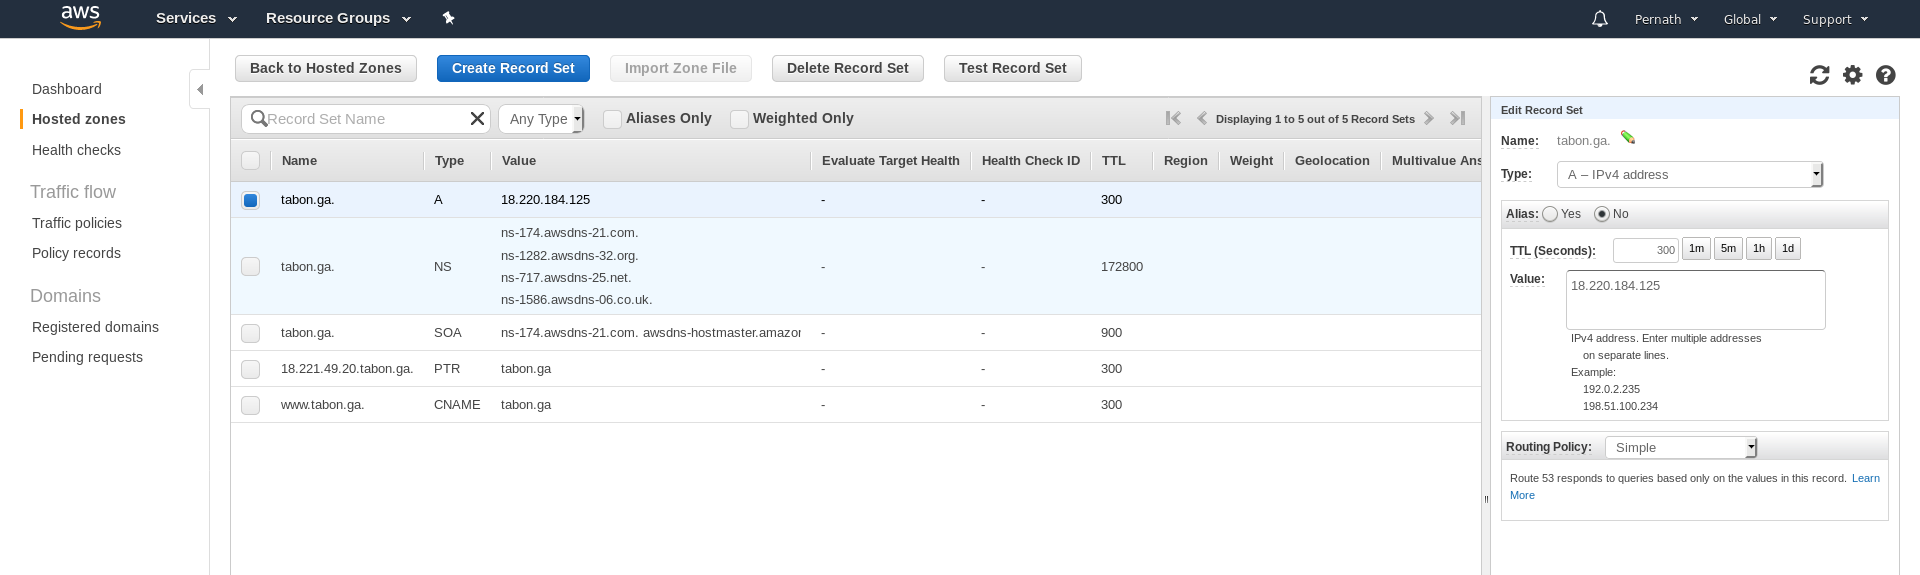
\includegraphics[width=\textwidth]{A}
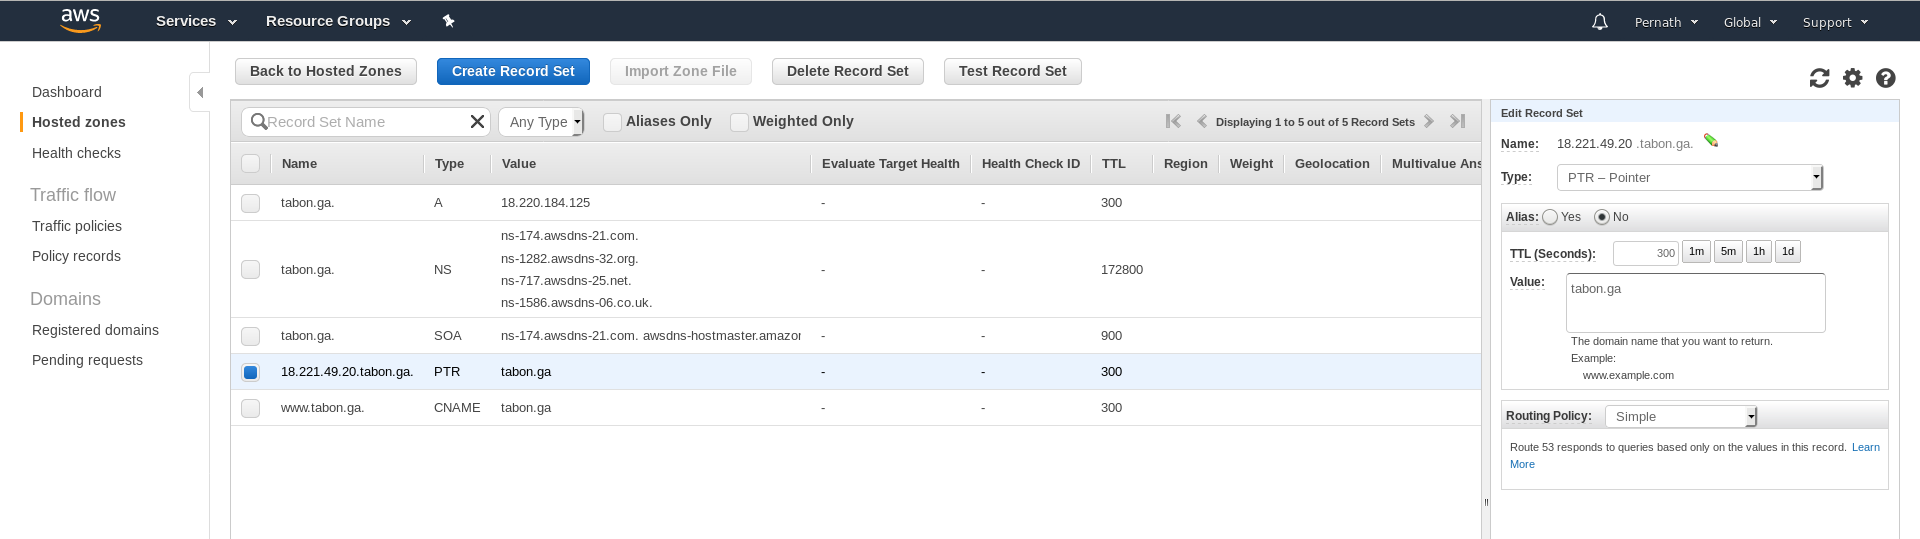
\includegraphics[width=\textwidth]{PTR}
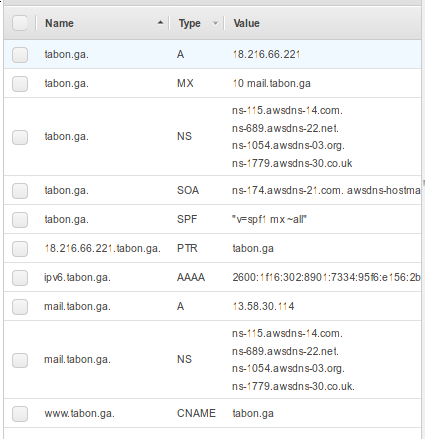
\includegraphics[width=\textwidth]{record_set}

\subsection*{Resumen de las configuraciones del servidor web y el servidor de aplicación y base de datos}
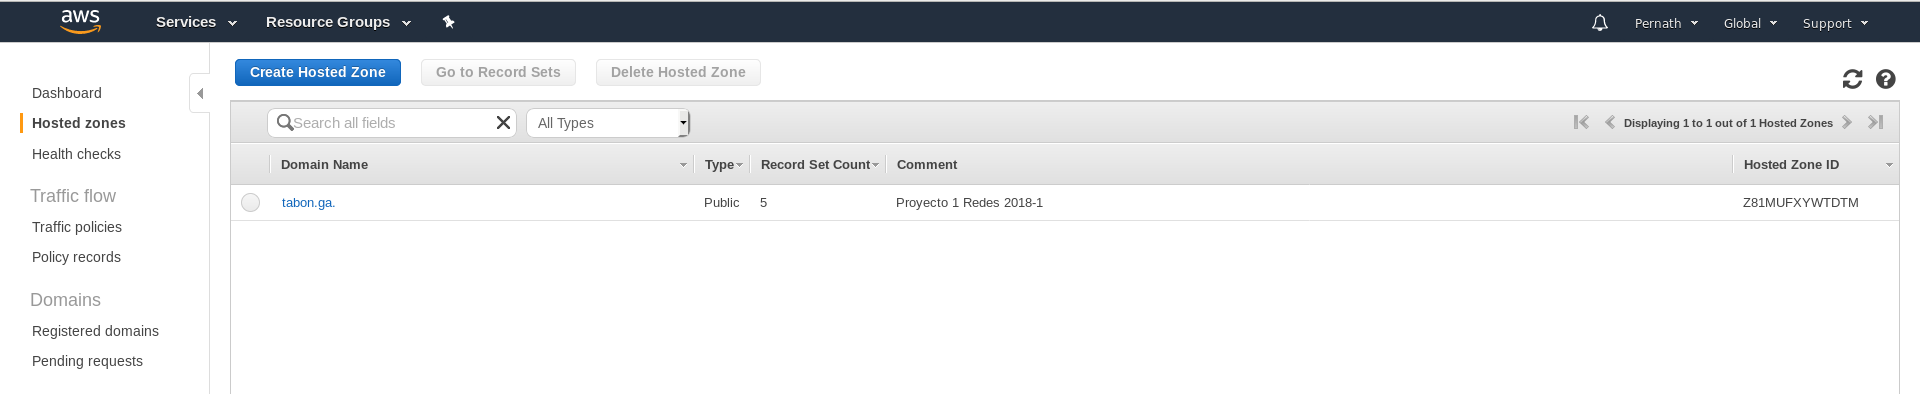
\includegraphics[width=\textwidth]{HostedZones}
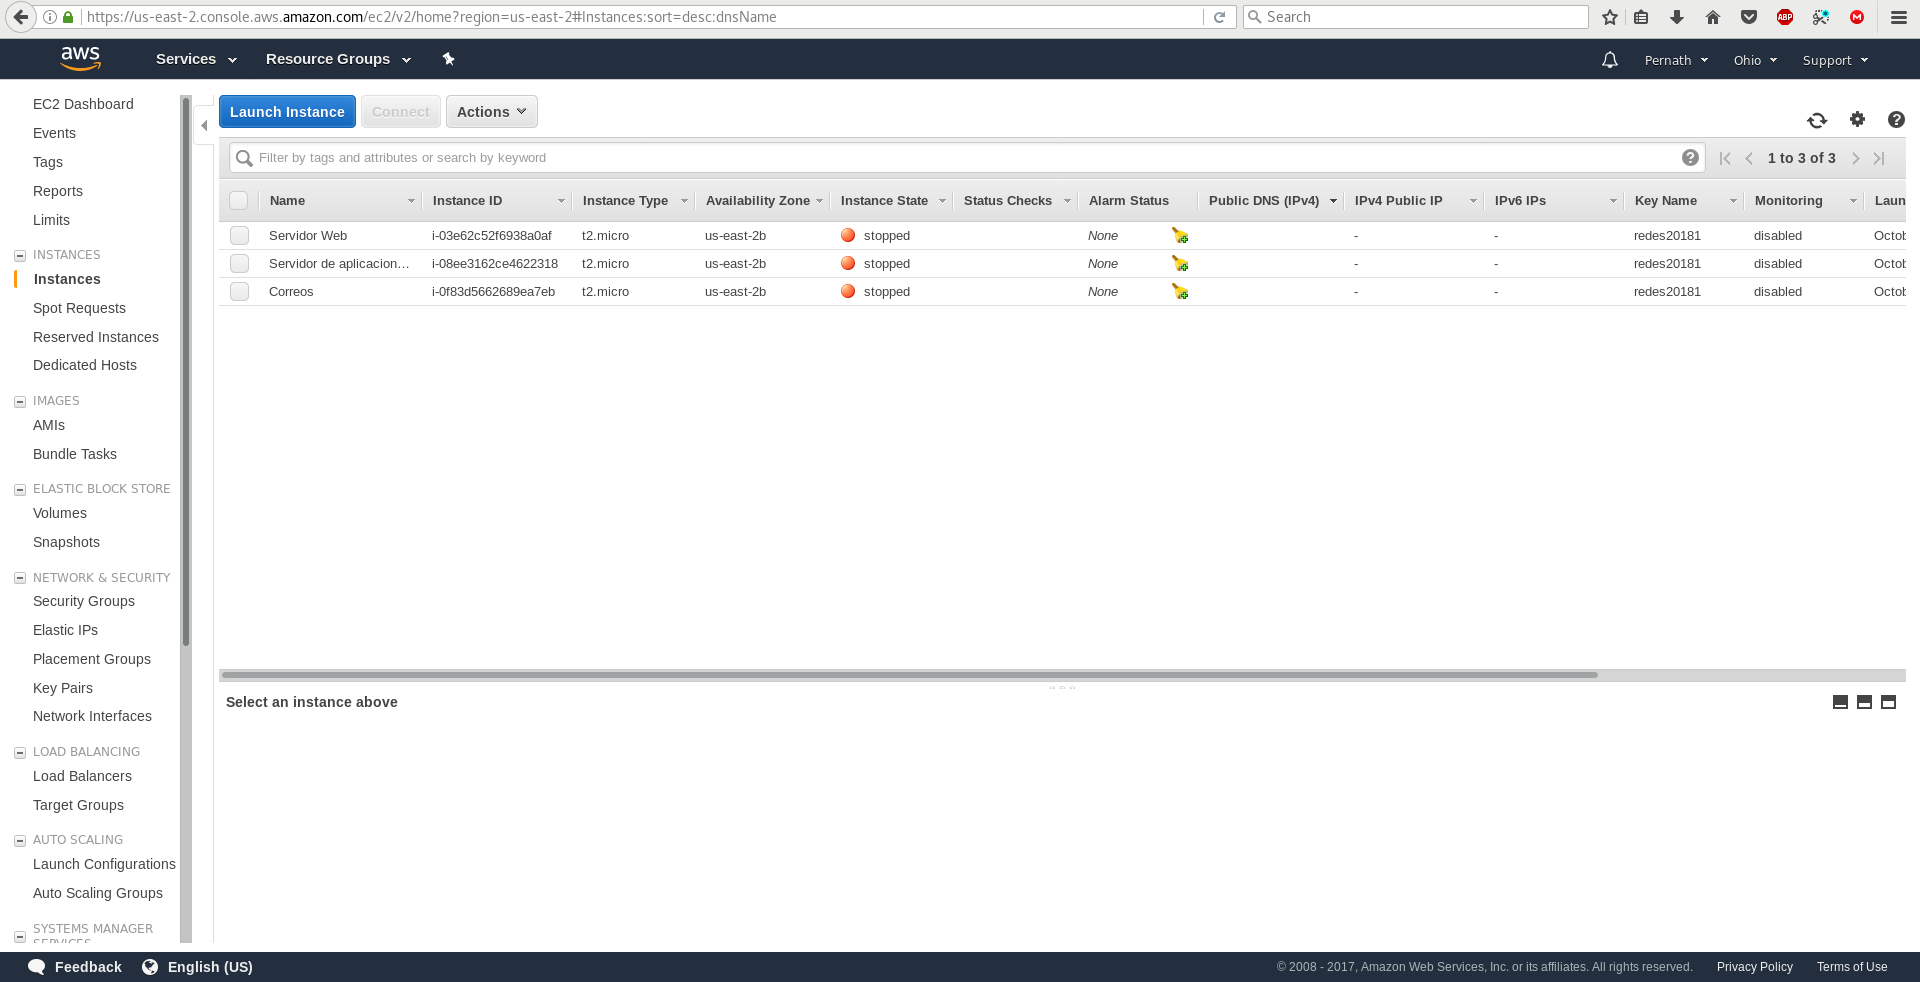
\includegraphics[width=\textwidth]{instances_dashboard}
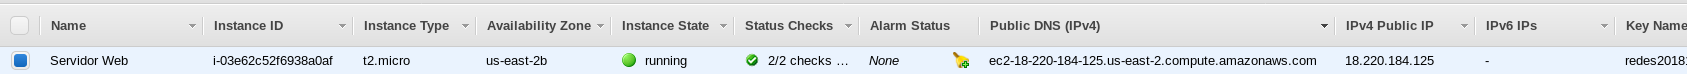
\includegraphics[width=\textwidth]{web_server}
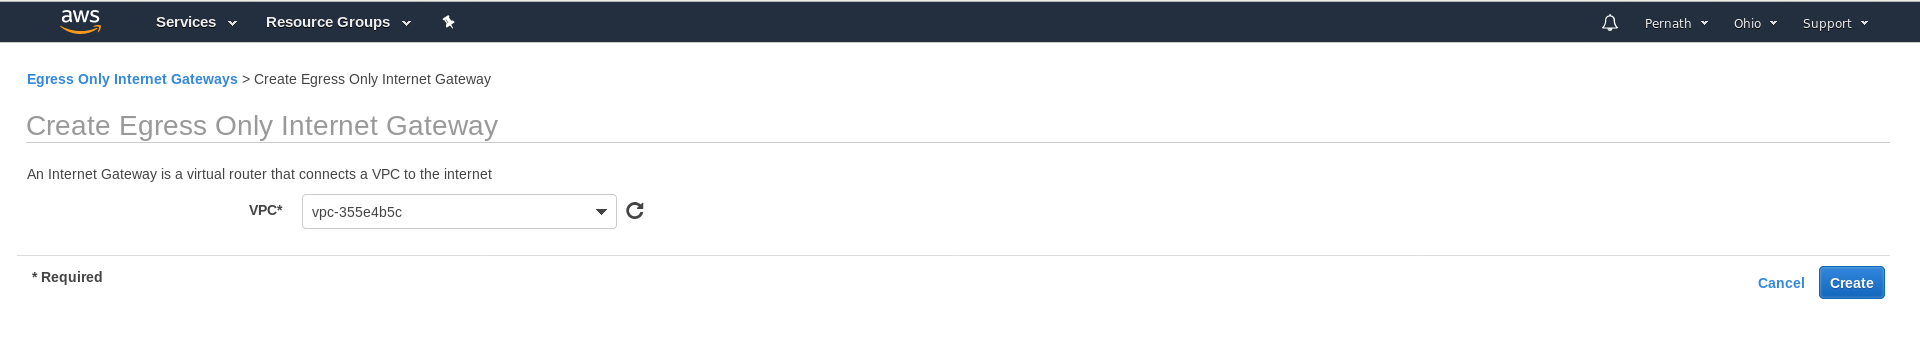
\includegraphics[width=\textwidth]{egress_only_gateway}
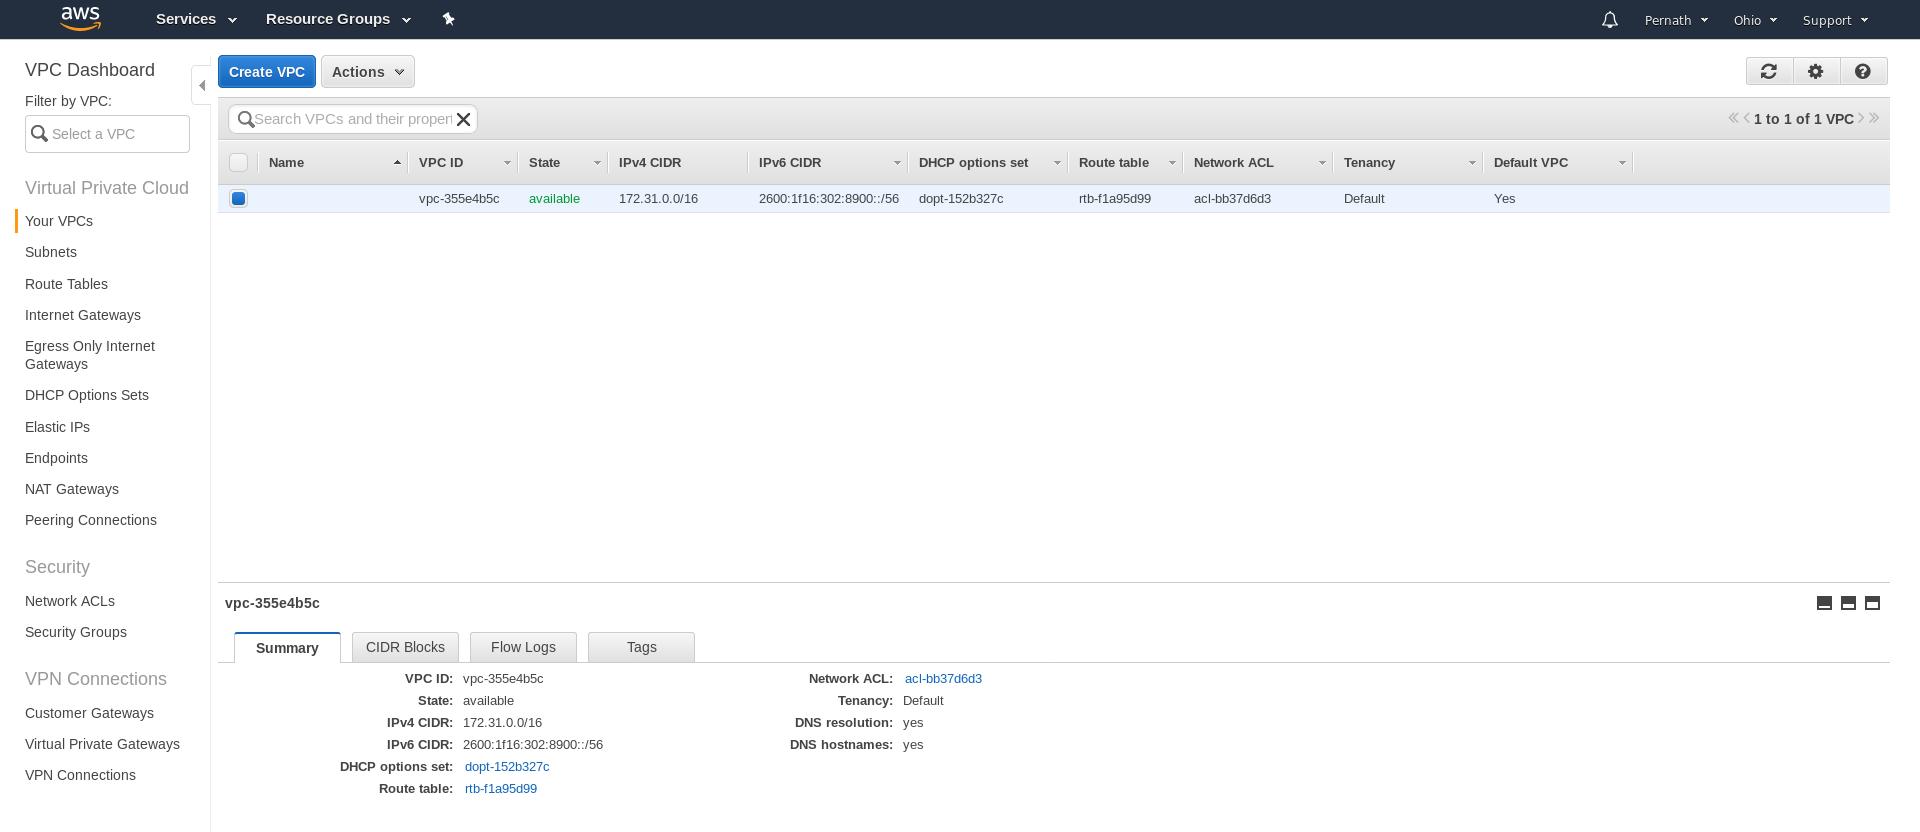
\includegraphics[width=\textwidth]{vpc}
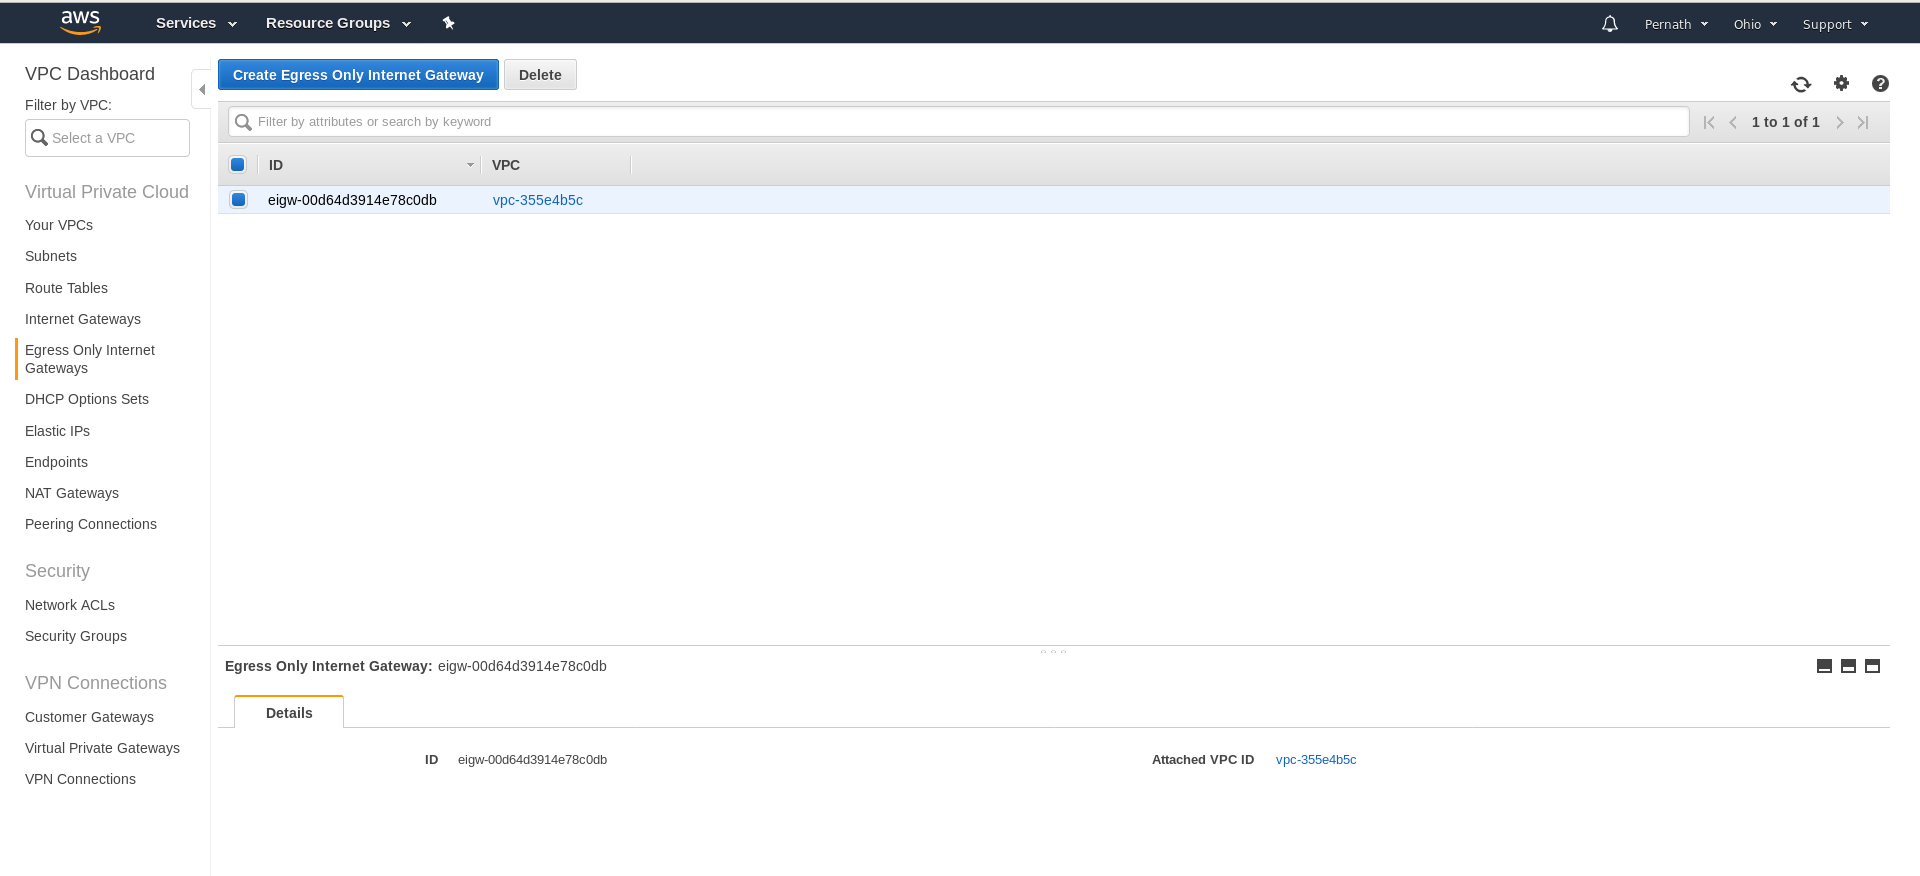
\includegraphics[width=\textwidth]{vpc_egress_only}
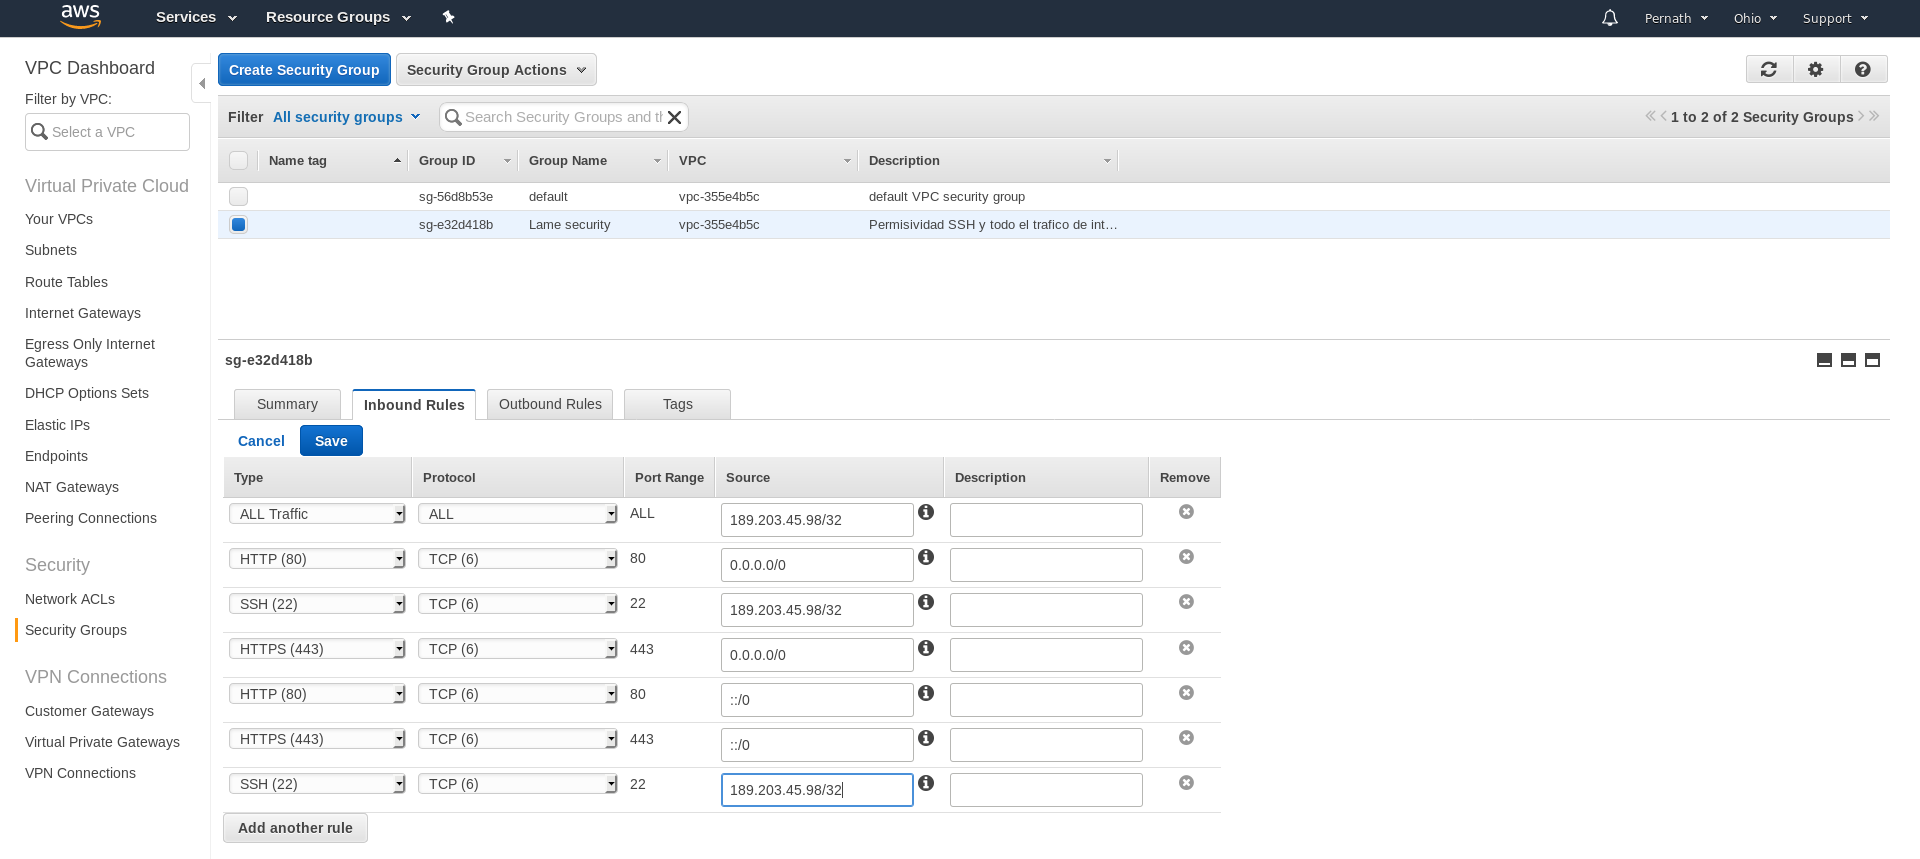
\includegraphics[width=\textwidth]{edit_security_group}
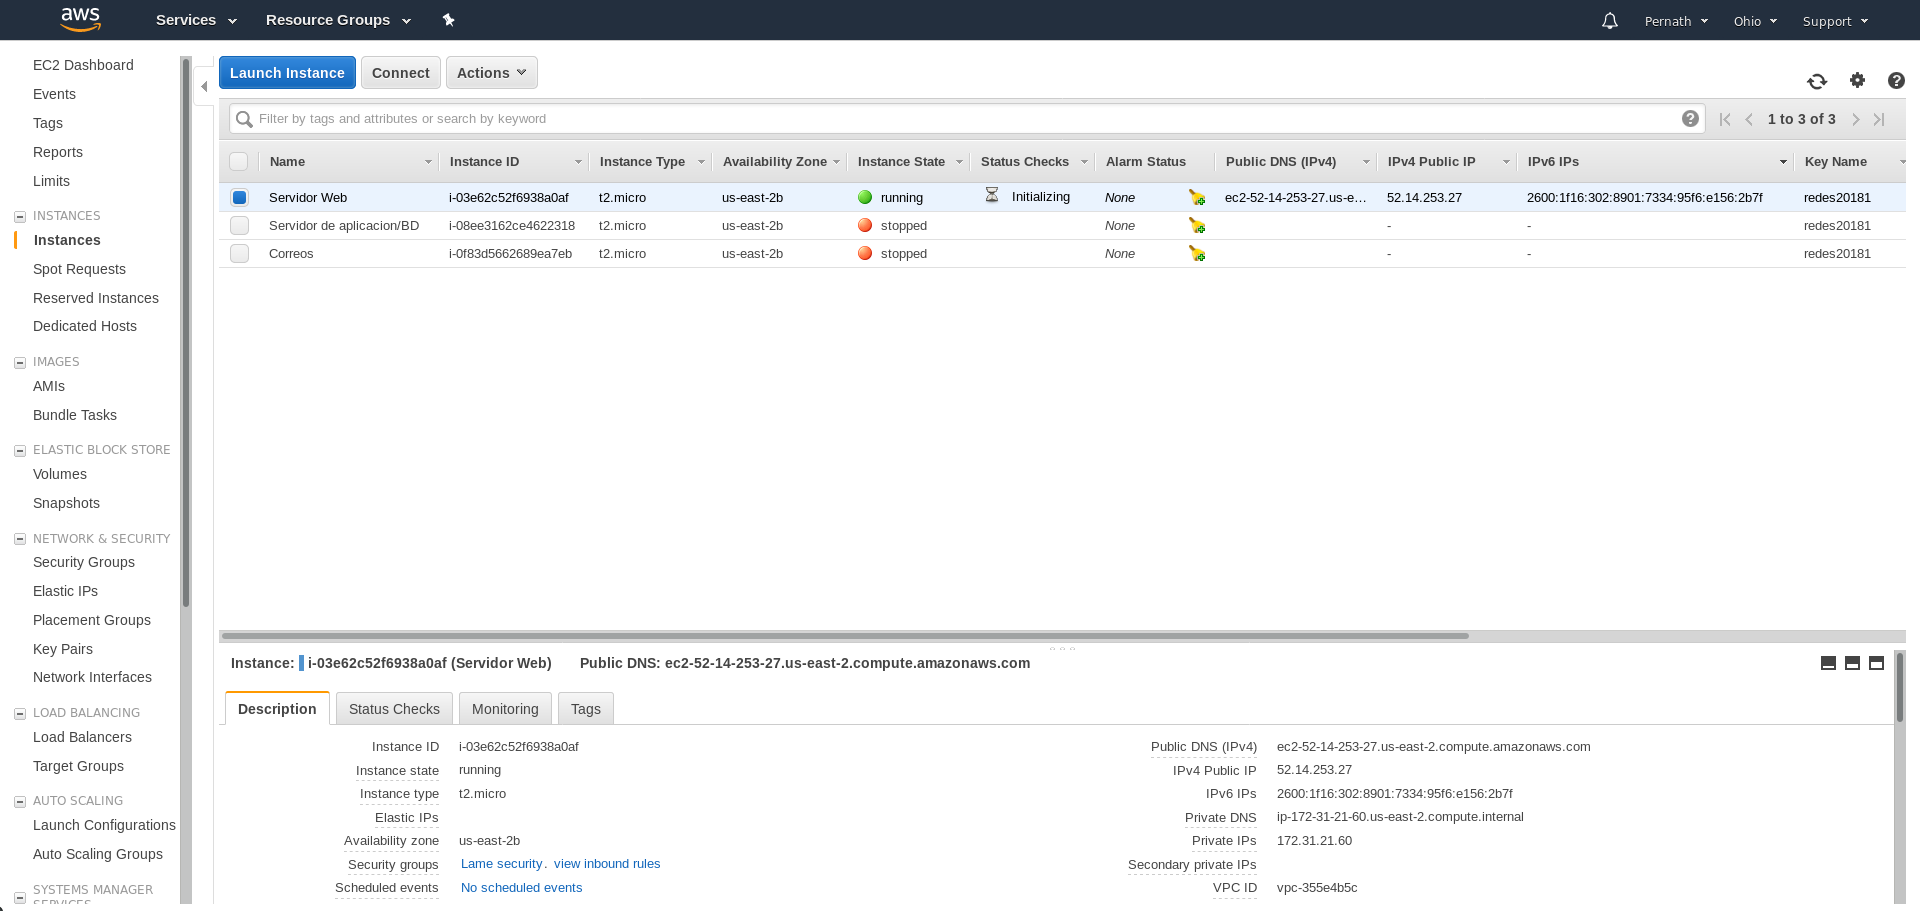
\includegraphics[width=\textwidth]{ipv6_assignment}
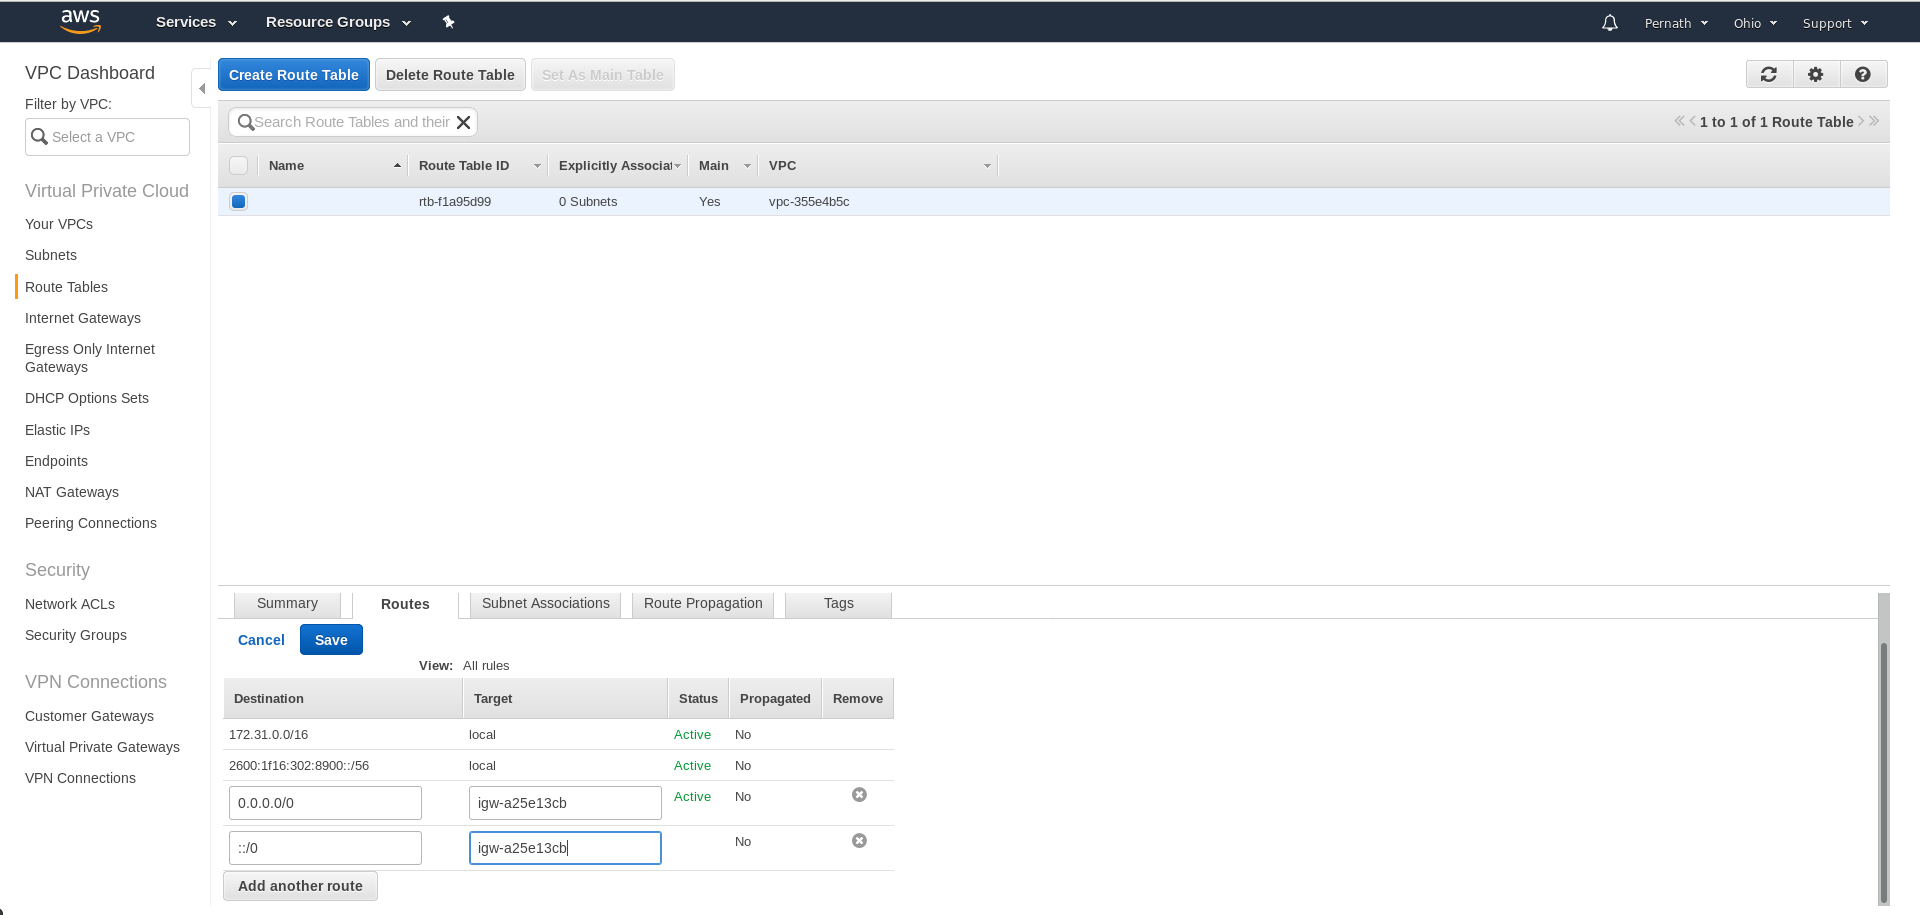
\includegraphics[width=\textwidth]{public_subnet}
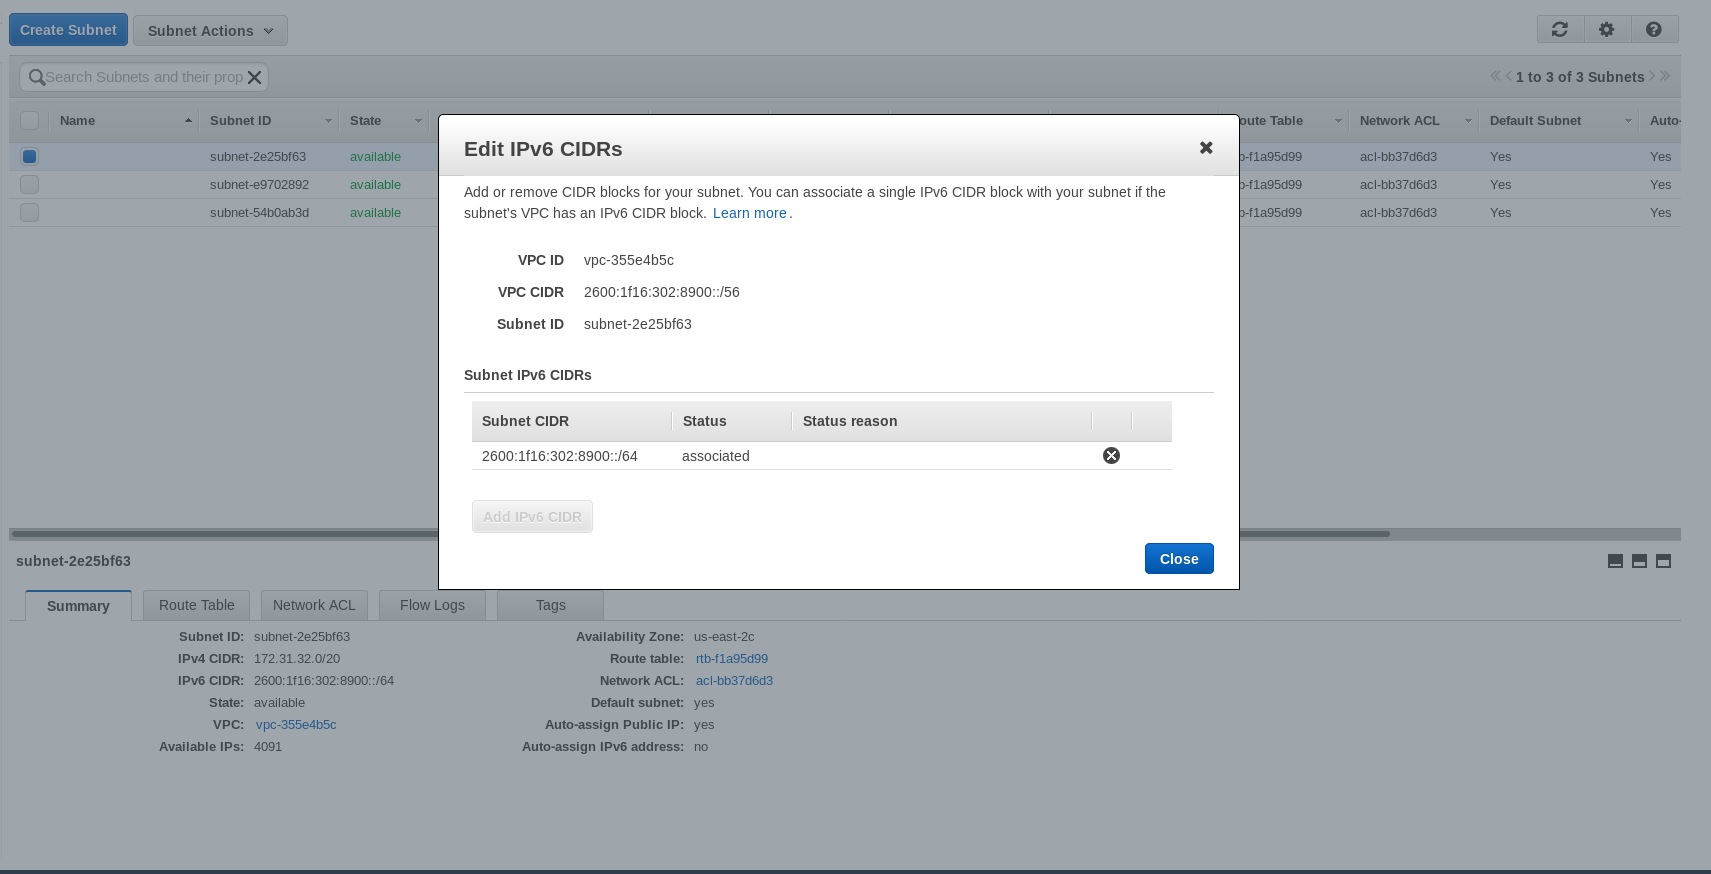
\includegraphics[width=\textwidth]{ipv6_cidr}
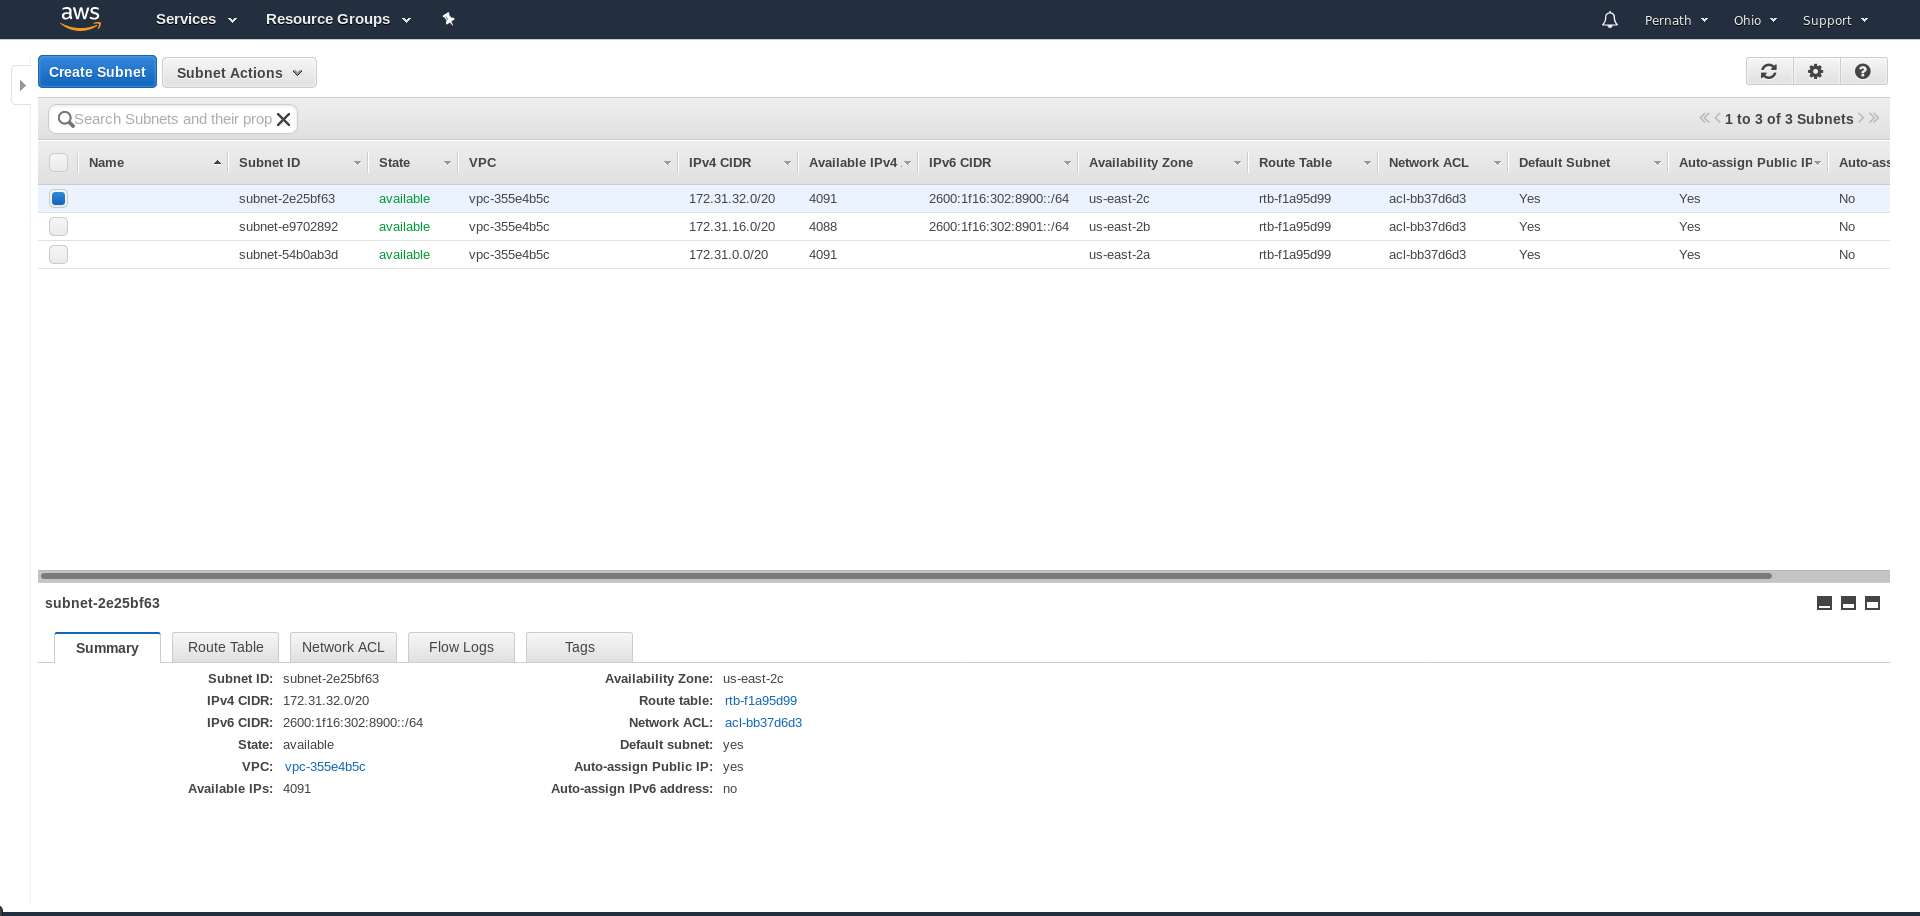
\includegraphics[width=\textwidth]{subnets}
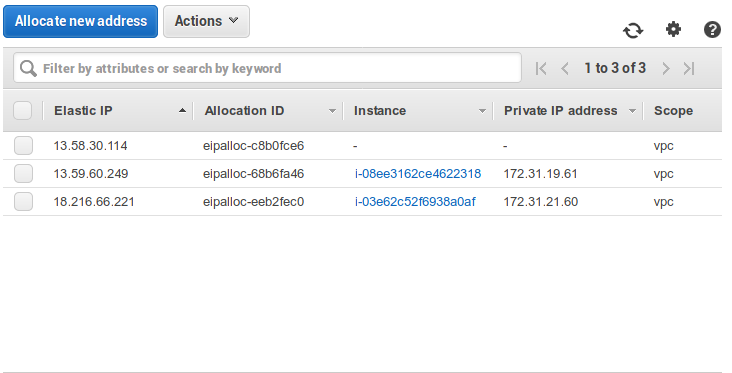
\includegraphics[width=\textwidth]{elastic_ip}
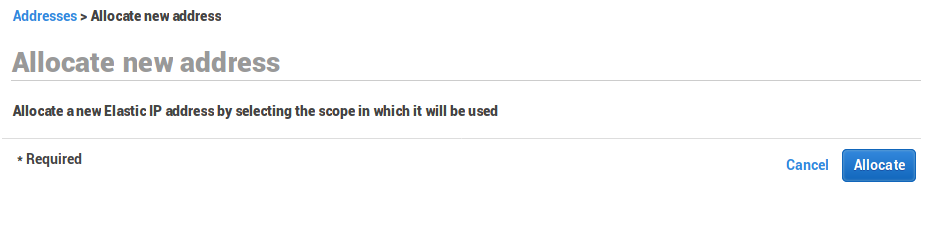
\includegraphics[width=\textwidth]{elastic_ip_allocate}
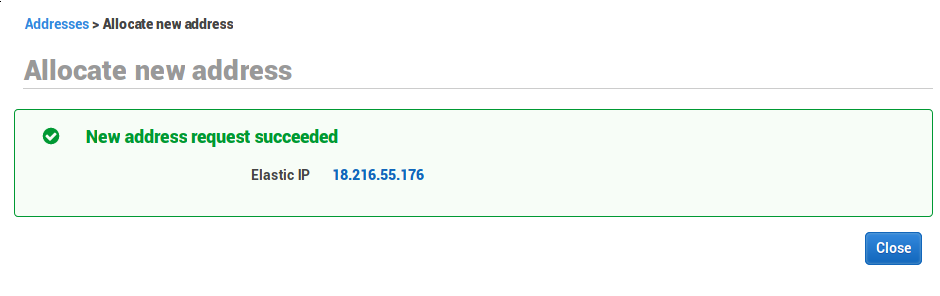
\includegraphics[width=\textwidth]{elastic_ip_success}
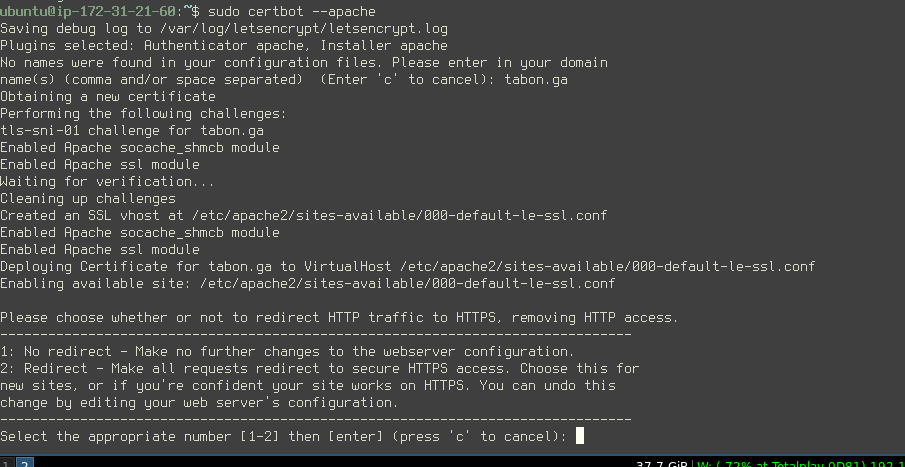
\includegraphics[width=\textwidth]{cert1}
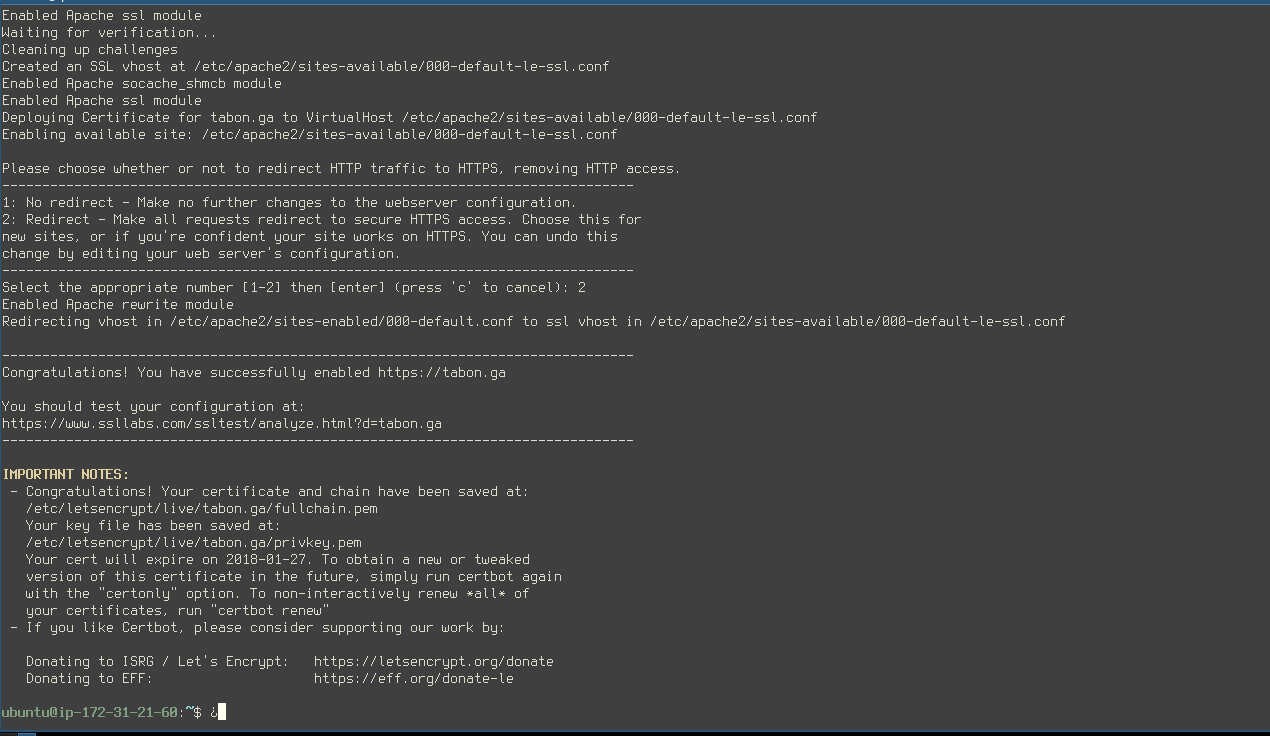
\includegraphics[width=\textwidth]{cert2}
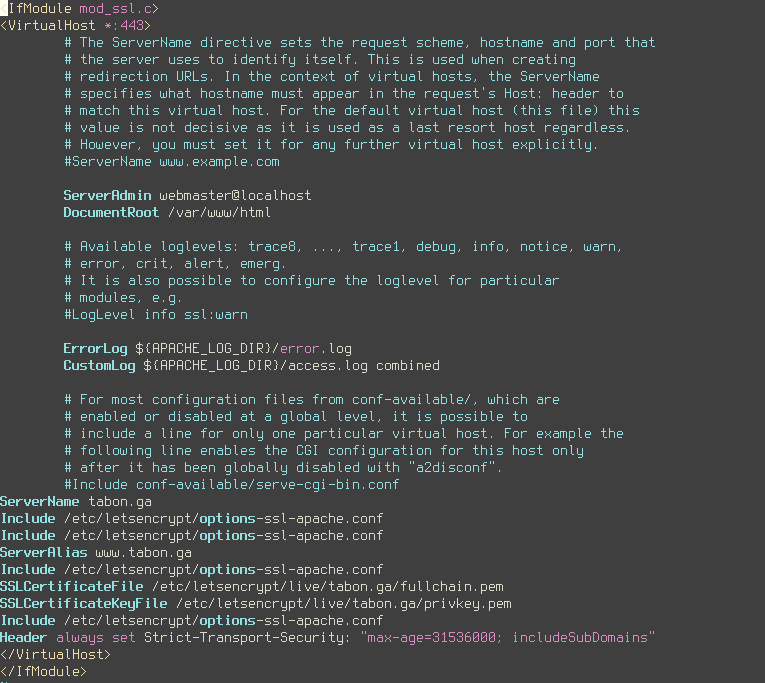
\includegraphics[width=\textwidth]{apache-ssl}
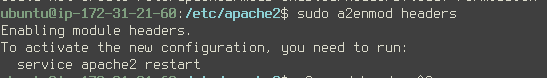
\includegraphics[width=\textwidth]{mods}
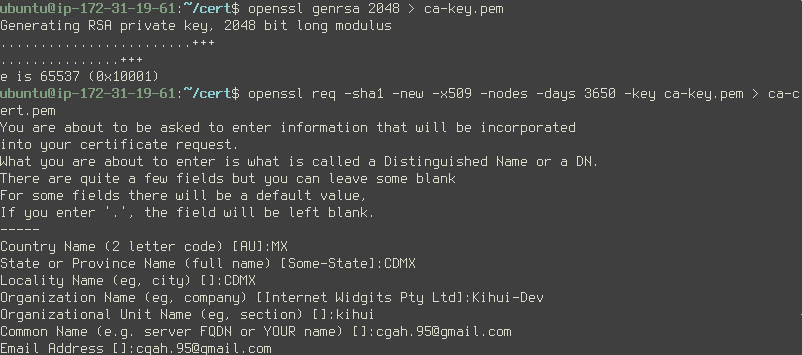
\includegraphics[width=\textwidth]{mysql_cert}
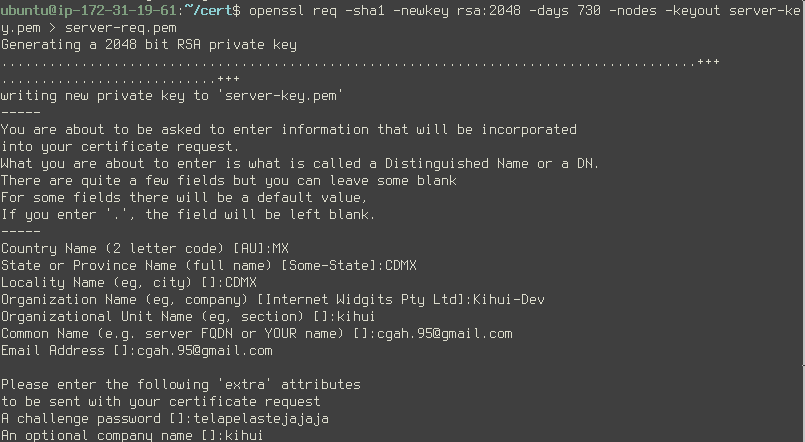
\includegraphics[width=\textwidth]{mysql_server-key}
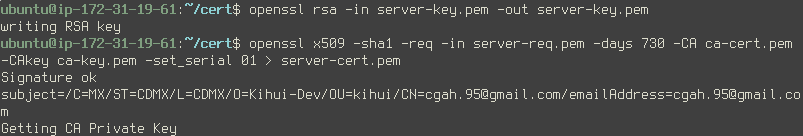
\includegraphics[width=\textwidth]{mysql_server-cert}
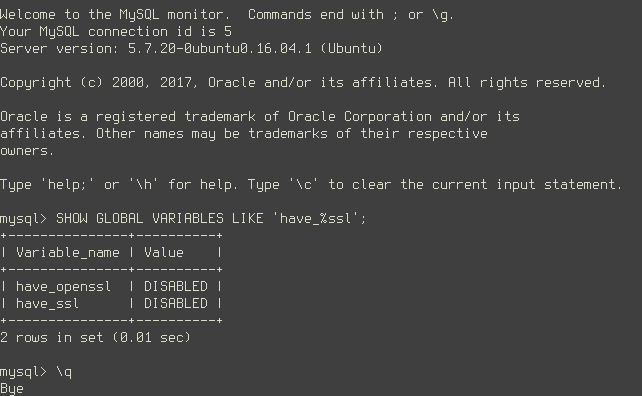
\includegraphics[width=\textwidth]{mysql_ssl-disabled}
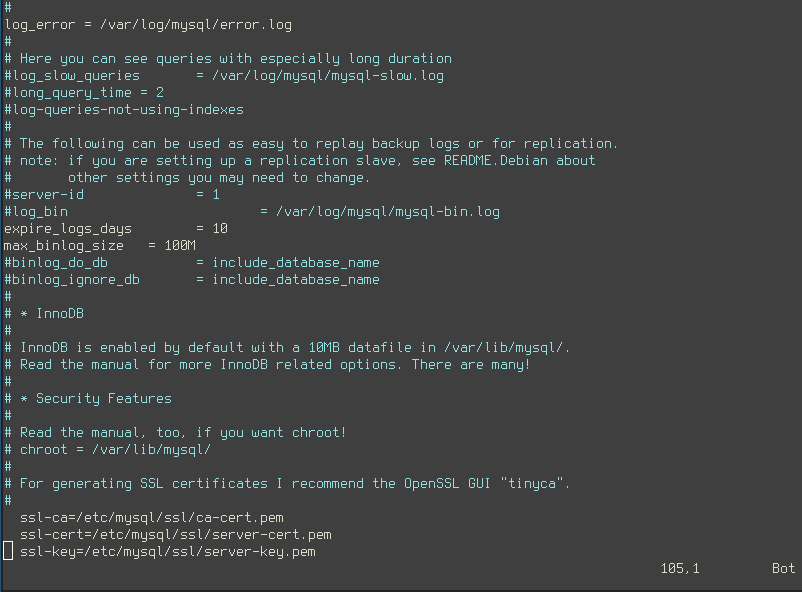
\includegraphics[width=\textwidth]{mysql_conf-ssl}
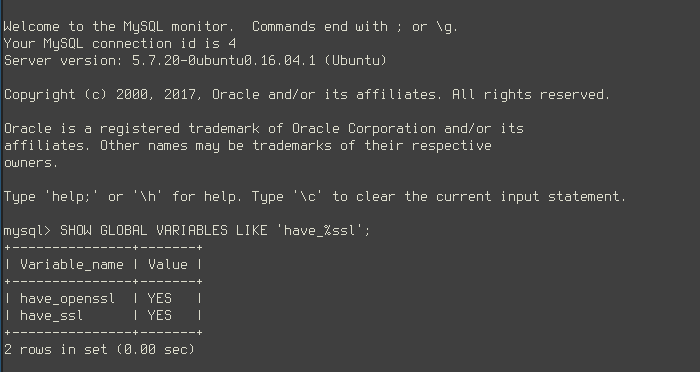
\includegraphics[width=\textwidth]{mysql_ssl-enabled}

\subsection*{Diagrama de la base de datos}
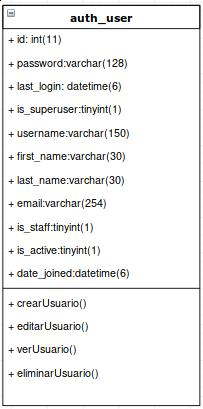
\includegraphics[width=\textwidth]{db}

\subsection*{Objetivo de la aplicación}
La aplicación fue desarrollada con el fin de ilustrar las funciones básicas de una aplicación web con base de datos, es decir, \textit{crear, editar, ver y liminar} y que pueden asociarse a distintos métodos HTTP de la capa de aplicación como PUT, POST, GET, PATCH o DELETE. \\
A partir de esta pequeña aplicación \textit{CRUD} puede escalarse a proyectos más grandes y de mayor complejidad, pues además sirve como aprendizaje para el desarrollador.
\subsection*{Uso de la aplicación}

\subsection*{Comentarios sobre el desarrollo del proyecto}
% We didn't deserve this
\end{document}
